\chapter{Methods and Implementation}
This chapter focuses on the experimental design and implementation of the artefact,
covering the self-imposed project management methodology, original concept design 
and the overall development process.

\section{Methodology}
When developing software, there are a wide variety of available options to manage the development 
process, which help to structure how time should be allocated as development progresses. 

\subsection{Waterfall} 
\para The first methodology considered was the Waterfall methodology, which is a very common 
approach to software development being sometimes referred to as the Software Development Life Cycle, or SDLC \autocite{adobePopularProjectManagement2023}.
Waterfall is a highly structured and strict methodology which enforces that one stage of development must be completed before the next can begin,
which creates a cascading set of steps, hence its namesake.

\begin{figure}[H]
    \centering
    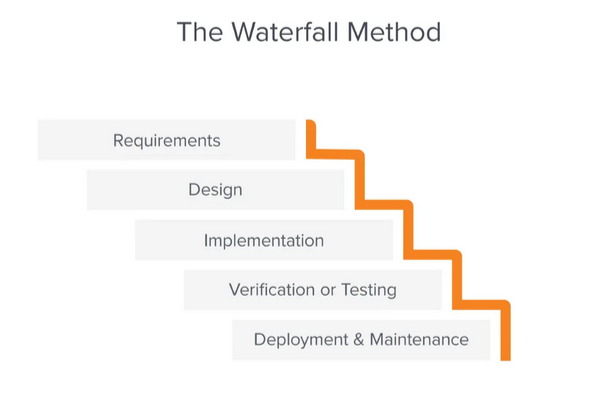
\includegraphics[width=0.8\textwidth]{Implementation/Methodology/Waterfall.png}
    \caption{An overview of a Waterfall workflow \autocite{adobeWaterfallMethodologyProject}. \label{fig:Waterfall}}
\end{figure}

\noindent Waterfall begins by ascertaining all project requirements for all stages of the project, which 
would include costs, risks, associated dependencies and overall timelines for completions of each stage.
Following this is the design stage, where a general high-level design is created to demonstrate the 
project, and this design is then acted upon and implemented in the implementation stage. Then, the 
implementation is rigorously tested before its eventual deployment.

\para It is a methodology with a strong reputation due to its clear structure, with all necessary facts and figures 
being calculated in the requirements stage before any designs or development occur. The clear structure allows 
progress to be easily measured against each predefined milestone.

\para Though, despite these advantages, Waterfall brings with it some clear disadvantages - the first of which 
being that with all requirements being defined at the very beginning of the project's development,
it introduces significant difficulty should there be any further requirements specified during development. This would also 
bring in the second disadvantage known as 'deadline creep' \autocite{adobeWaterfallMethodologyProject}; 
if one stage is delayed, such as by request for additional features, this would then impact all subsequent stages. 

\subsection{Agile}
The second methodology considered was another highly reputed software development methodology known as Agile.


\subsection{Comparison}